\section{Does Sensitivity Convert into Upgrade Value?}
\label{sec:r4}

\begin{figure}[t]
\centering
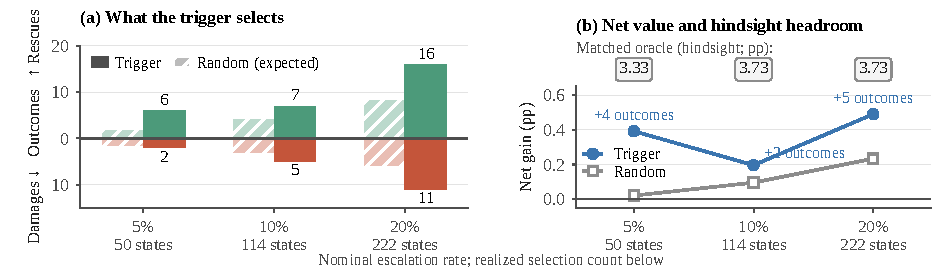
\includegraphics[width=\columnwidth]{figures/f4_trigger_oracle.pdf}
\caption{Sensitivity versus benefit, by escalation budget, on held-out ordinary states (1020 U1 rows; 38 rescues, 31 damages): a frozen Q-only uncertainty trigger, matched-count random selection (expected), a hindsight oracle with the same per-cell counts, and a faint post-hoc KL$(\mathrm{B}\|\mathrm{Q})$ reference (needs BF16). (a)~Net gain, (rescues $-$ damages)/1020, pp. (b)~Share of the 69 outcome-changing states selected; black: the most any selection with the same per-cell counts can capture. Values: Table~\ref{tab:oracle}.} % src: analysis/fork/out/oracle_trigger_20261002T024423Z.json; analysis/fork/out/oracle_trigger_20261002T024423Z.md; analysis/fork/out/token_mech_20261002T003130Z.json
\label{fig:oracle}
\end{figure}

\S\ref{sec:value} and \S\ref{sec:sameprec} show that outcomes are sensitive to the action and that sensitivity alone does not identify a need for more bits. Three tests ask whether a measure of numerical error, or a signal visible to Q, tells which changes are worth making: an error dose, a fidelity diagnostic on shared states, and a frozen trigger.

\paragraph{Error dose: trajectory divergence and success respond differently.} Scaling the quantizer's own weight error, $W_\alpha=W+\alpha(W_{\mathrm{Q}}-W)$ with $\alpha\in\{0, 0.25, 0.5, 1, 2\}$ (exploratory; not a bit width), lowered agreement with BF16's actions at every step of $\alpha$ in all six cells (in q8 RTN-W3, the share of BF16's decisions before the first differing action is 1, 0.32, 0.16 and 0.04 at $\alpha=0$, 0.25, 0.5 and 1). Success did not follow: no success step up to $\alpha=0.5$ is resolved under both intervals, and a fall in success between $\alpha=0.5$ and 1 is resolved only in RTN-W3 ($-20.8$ and $-14.1$\pp{} in q4 and q8; Appendix Table~\ref{tab:dose}). % src: analysis/fork/out/backfill_20261003T193042Z.md (TL;DR 2; §2); docs/insights/PERTURBATION_PROTOCOL.md §2.2

\paragraph{KL diagnostic: fidelity tracks whether the action changes, not yet what the change does.} Methods of one model are compared on ordinary BF16-sourced states (U2B, shared by every method; they follow the BF16 policy's state distribution) by $D_{cc}=\YY{QB}-\YY{BB}$, Q's action against B's under the shared BF16 continuation (Appendix~\ref{app:panels}). % src: docs/insights/NEWMETHOD_PANEL_PROTOCOL.md (§2.1, §4)
Of two rotation-based quantizers \citep{ashkboos2024quarot,liu2025spinquant}, SpinQuant-W4A4 is closer to BF16 than QuaRot-W4A4 on the shared q8 states (mean teacher-forced approximate token KL, Appendix~\ref{app:panels}: 0.165 against 0.199), but its task value is not shown to differ: the pre-registered matched contrast is $+1.2$ [$-3.9$, $+6.2$]\pp{} (Holm-adjusted $p=1.0$; one block rests on a re-run). % src: analysis/fork/out/newmethod_q8_20261004T051538Z.md; analysis/fork/out/newmethod_q8_20261004T051538Z.json (tau2.contrasts; fidelity.cells.*.KLu_mean); docs/insights/NEWMETHOD_PANEL_PROTOCOL.md (A1.2, A7)
A diagnostic decomposition on the same 255 states (exploratory, post hoc; $t$ over three block differences) resolves the KL gap ($-34$ [$-57$, $-11$]$\times10^{-3}$), while differences in the action-difference rate ($+0.8$ [$-11.4$, $+13.0$]\pp{}) and the flip rate given a difference ($+2.7$ [$-10.2$, $+15.3$]\pp{}) remain unresolved. Across the eleven q8 cells (Spearman, descriptive), mean KL is strongly related to the action-difference rate ($\rho=0.99$) and, through it, to B's rescues and damages together ($0.81$ and $0.93$); its relations with the flip rate given a difference ($0.46$) and the net $D_{cc}$ ($-0.44$) are weaker and less consistent. Within cells it separates differing from identical actions (mean AUC 0.93) far better than flips among them (0.46, an average over configurations). Numerical fidelity thus discriminates well whether the action changes, but has not yet shown reliable predictive power for what the change does to the task (Appendix~\ref{app:panels}). % src: analysis/fork/out/kl_decomp_20261005T000559Z.md (TL;DR; §2; §3); analysis/fork/out/kl_decomp_20261005T000559Z.json

\paragraph{Frozen trigger.} $G$, $H$ and $F$ require running B and all four branches; a deployable rule sees only Q. We test whether a Q-only signal that finds outcome-changing decisions also finds the ones worth upgrading.
Scored at the token level on one development block, Q's entropy at the start of its action separates states where B and Q act differently from states where they act identically (AUC 0.66--0.91 per sub-bank and model), but among states where the actions differ, no Q-visible statistic reliably separates flips from non-flips (Appendix~\ref{app:token}). % src: analysis/fork/out/token_mech_20261001T185031Z.md (§1a, §1b)
We then froze a Q-only trigger on that block before any later state was scored: escalate one decision when the minimum Q margin over its action is low (margins predict cross-precision divergence; \citealp{du2026greedy}), with per-cell thresholds at 5, 10 and 20\% escalation rates. On two held-out blocks (1020 rows, 69 outcome-changing states) it captured 8, 12 and 27 outcome-changing states, against 3.48, 7.52 and 14.30 expected at random ($p=.0182$, $.0613$, $.0002$; Figure~\ref{fig:oracle}b). % src: analysis/fork/out/token_mech_20261002T003130Z.md (§3 Validation, U1 S_mm PRIMARY)

\paragraph{It does not yet select net-beneficial replacements.} The captured states were rescues and damages alike (6/2, 7/5 and 16/11), for net gains of $+4$, $+2$ and $+5$ against random expectations of $+0.21$, $+0.98$ and $+2.38$ (exact one-sided $p=.0345$, $.417$, $.262$); no level was fixed in advance, and the 5\% rate does not survive Holm correction. A hindsight oracle with the same per-cell counts nets $+3.33$, $+3.73$ and $+3.73$\pp{} (Figure~\ref{fig:oracle}a). This headroom is positive by construction, because the oracle picks only rescues and never a damage; the trigger captures 4/34, 2/38 and 5/38 of it. A post-hoc KL$(\mathrm{B}\|\mathrm{Q})$ score, which needs BF16, also captures turnover above chance without a significant net gain (Appendix~\ref{app:oracle}). % src: analysis/fork/out/token_mech_20261002T003130Z.md (§3 Validation, U1 S_mm PRIMARY); analysis/fork/out/oracle_trigger_20261002T024423Z.md (§1a, §2)
The held-out blocks reuse the development tasks. A learned router trained on task reward \citep{li2026dynamicmp} is not tested here.

